\documentclass[pdfa,cucitura]{toptesi}

\hypersetup{
    pdfpagemode={UseOutlines},
    bookmarksopen,
    pdfstartview={FitH},
    colorlinks,
    linkcolor={blue},
    citecolor={red},
    urlcolor={blue}
}

%
% Phantom space for abbreviations
%
\usepackage{xspace}
%
% To insert doi identifiers
%
\usepackage{doi}
\renewcommand{\doitext}{DOI }
%
% Improve citations from biblio
%
\usepackage{cite}
%
% This is to create hyperlinks for index, URLs and citations
% (now we can use the command \url{...} to create URL with hyperlink)
% 
%\usepackage{color}
%\usepackage[a4paper,colorlinks=true,urlcolor=blue,citecolor=blue,linkcolor=blue,bookmarks=false]{hyperref}
%
% For pasting text files
%
%\usepackage{fancyvrb}
%
% Used to express formulas like n^th
%
%\usepackage{mathtools}
%
% For table formatting
%
%\usepackage{longtable}
%\usepackage{makecell}
%\usepackage{multirow}
%
% For plotting results
%
%\usepackage{pgfplots}
%\pgfplotsset{compat=newest}
%
% For placing floats
%
%\usepackage{placeins}
%
% For subfigure environment
%
\usepackage{subcaption}
\usepackage{cleveref}
\captionsetup[subfigure]{subrefformat=simple,labelformat=simple}
\renewcommand\thesubfigure{(\alph{subfigure})}
%
% For Appendix section
%
%\usepackage[titletoc,toc,title]{appendix}
%
% Definition of margins
%
%\usepackage[top=2cm,bottom=2cm,left=2cm,right=2cm]{geometry}
%
% Paragraph skip and indent
%
%\setlength\parskip{\medskipamount}
%\setlength\parindent{0pt}
%
% For itemize and enumerate spacing
%
\usepackage{enumitem}
%
% For International System of Units (SI)
%
%\usepackage[binary-units]{siunitx}
%\sisetup{per-mode=symbol} % 1/s instead of s^-1
%
% For programming code
%
\usepackage{listings}
\lstset{
basicstyle=\ttfamily,
columns=fullflexible,
xleftmargin=3ex,
breaklines,
breakatwhitespace,
escapechar=`
}

% Some page parameters
\setlength{\parskip}{\medskipamount}
% Horizontal rule
\newcommand{\HRule}{\rule{\linewidth}{0.2mm}}


%
% Frequently used abbreviations.
% - example: \ie this is an example
%
\def\eg{e.g.\xspace}
\def\ie{i.e.\xspace}
\def\chap{Chapter\xspace}
\def\sec{Section\xspace}
\def\myfig#1{Fig.~#1\xspace} % usage: \myfig{\ref{fig:tag}}
\def\mytab#1{Tab.~#1\xspace}
\newcommand{\ltx}{\LaTeX\xspace}
\newcommand{\txw}{TeXworks\xspace}
\newcommand{\mik}{MikTex\xspace}
\newcommand{\html}{HTML\xspace}
\newcommand{\xhtml}{XHTML\xspace}
\newcommand{\cmd}[1]{\texttt{#1}\xspace}

% Styles
\newcommand{\itemname}{\textbf}
\newcommand{\thead}{\textbf}

% To cite RFC, es. \rfc{822}
\newcommand{\rfc}[1]{RFC-#1\xspace}
% To cite file (es. \file{autoexec.bat}) or fake URI (i.e. \file{http://www.lioy.it/})
% for real URIs use \url o \href
\newcommand{\file}[1]{\texttt{#1}\xspace}
% For inline code
\newcommand{\code}[1]{\lstinline|#1|}
% Backslash
\newcommand{\bs}{\textbackslash}
% Term definition with insertion into the index
\newcommand{\tdef}[1]{\textit{#1}\index{#1}}
% Meta-term
\newcommand{\meta}[1]{\textit{#1}}


\begin{document}
\selectlanguage{english}

\CorsoDiLaureaIn{Corso di Laurea Magistrale in }
\TesiDiLaurea{Master Thesis}
\AdvisorName{Supervisor}
\CandidateName{Candidate}


\logosede{res/logopolito}
\ateneo{Politecnico di Torino}

\titolo{Pin Control Protection}
\sottotitolo{Protecting Linux Kernel Pin Control Subsystem from Pin Control Attack}

\corsodilaurea{Ingegneria Informatica}

\candidato{Andrea \textsc{Genuise}}

\relatore{prof.\ Antonio Lioy}

\sedutadilaurea{\textsc{Academic~Year} 2016-2017}


\errorcontextlines=9

\frontespizio
\paginavuota
\newpage

\advance\voffset -5mm
\advance\textheight 30mm


\begin{dedica}
\textdagger\ A nonno Carmelo
\end{dedica}


\sommario

Recently embedded systems have become more and more integrated with all aspects of our lives, and their security concerns have risen as well.
They spread in various fields such as automotive, electronic devices, home automation, manufacturing and mission critical applications. These systems, in particular PLCs
deployed within the context of an Industrial Control System, use Input/Output interfaces to interact with the physical world by means of sensors and actuators.
As demonstrated by a novel kind of attack called Pin Control Attack, one can tamper with the integrity or the availability of legitimate I/O operations,
factually changing how a PLC interacts with the outside world and possibly causing physical damage to people and environment.
In this thesis we design a possible countermeasure to the attack and implement it for Linux Kernel on an ARM-based Programmable Logic Controller,
showing its effectiveness and impact on PLCs which usually have very limited resources and strict timing requirements.


\ringraziamenti

TODO Acknowledgements.


%\tablespagetrue
%\figurespagetrue

\indici

\mainmatter


\section{Introduction}

TODO Introduction.


\chapter{Related work}
\label{chap:related}

In this chapter we summarise the state of the art about security of embedded systems at the time of writing.
First, we discuss about the attacks of the recent years, showing how the embedded systems security concerns are rising.
Next, we analyse the defense mechanisms currently available in the literature, realising that they are still in a very early stage of their life.
Finally, we consider the existing attacks and defenses targeting the hardware level, as Pin Control Attack does,
showing that they are currently not applicable to embedded systems.


\section{Attacks}

In the past few years we have seen several attacks targeting embedded systems: most notably the infamous Stuxnet \cite{stuxnet} targeting an Iranian nuclear facility in 2010.
More recently Grandgenett et al. \cite{io-command} analysed the authentication protocol between the RSLogix 5000 software and the PLC, based on a simple challenge-response mechanism.
Since the protocol lacks freshness in its messages, is vulnerable to replay attacks, through which an attacker could repeat privileged commands to the PLC.
Furthermore, they found that both the decoding of the challenge and the encoding of the response use an RSA-2048 key which is hard-coded in the RSLogix software,
and it is actually valid for any Rockwell/Allen Bradley PLC.
This indicates how the security mechanisms of these systems often have a really poor design, if any.

Papp et al. \cite{taxonomy} analysed the existing attacks on embedded systems, relying on the proceedings of security conferences, with a focus on computer hacking,
and on the Internet for media reports, blogs and mailing list.
They built a taxonomy based on five dimensions: precondition, vulnerability, target, attack method and effect of the attack,
showing that the threats to embedded systems are similar to the ones that affect traditional IT systems.
However, embedded systems still lack solutions and tools to address these issues, and many ongoing research efforts are trying to deploy and adapt them to the needs of this field.

For our purpose, we may classify the attacks found in literature using a simpler criterion based on the attack method. We may distinguish three main categories:
\begin{enumerate}
	\item \itemname{Firmware modification}: all the attacks aiming to upload a malicious firmware version (or part of it) in the device belong to this category.
	\item \itemname{Logic modification}: this category consists of the attacks that modify the PLC logic in some way. In this case the integrity of the firmware is not violated,
		but a malicious program, or logic, is inserted into the PLC to make it misbehave during the control process.
	\item \itemname{Control flow modification}: it includes the attacks that alter the normal control flow of a process by leveraging classic programming vulnerabilities
		such as buffer overflow or expired pointer dereference.
\end{enumerate}

We briefly report about these different kind of attacks in the following sections.


\subsection{Firmware modification attacks}

Almost all modern embedded systems provide a way to update the firmware, and the attackers could exploit this feature to upload its own malicious firmware.
Basnight et al. \cite{firmware-mod} reverse engineered an Allen-Bradley ControlLogix L61 PLC firmware showing how to bypass the
firmware update validation method and successfully upload a counterfeit firmware.
Peck et al. \cite{ethernet-vuln} demonstrate how using commonly available software an attacker can write and load his malicious firmware into Ethernet cards of devices
used in control systems, potentially infecting the entire industrial control system.
Cui et al. \cite{print-vuln} discovered a vulnerability in the HP-RFU (Remote Firmware Update) feature of LaserJet printers,
that allows remote attackers to make persistent modifications to the printer's firmware by simply printing to it.


\subsection{Logic modification attacks}

Stuxnet \cite{stuxnet} belongs to this category. Along with its several components, mainly used to replicate and control the malware,
its core is essentially an infected version of a SCADA software library used to program the PLC itself.
By hooking some of the library functions it is able to load infected code and data blocks into the PLC and hide itself from the operator.
McLaughlin et al. \cite{dynamic-payload,sabot} evaluated some techniques and implemented a tool (SABOT) to infer the structure of a physical plant and craft a dynamic payload,
allowing an attacker to cause an unsafe behaviour without having a deep \emph{a priori} knowledge of the target physical process.
Similar techniques might mitigate the precondition needed by an attack, making it even more viable.
Beresford \cite{siemens-s7} showed how the PLCs and the protocols used for communication in control systems were built without any security in mind,
and demonstrated that they are affected by many vulnerabilities which may also enable the attacker to know the current configuration and rewrite the PLC logic.
More recently, Klick et al. \cite{plc-network} used an internet-facing PLC as a network gateway by prepending a backdoor, made of a port scanner and a SOCKS proxy,
to the existing logic code of the PLC. They developed a proof-of-concept tool called \emph{PLCInject} to demonstrate their approach and measure the effects on the network.


\subsection{Control flow modification}

Many recent advisories \cite{abb-codesys,codesys-server,schneider-bof,rockwell-vuln,rockwell-vuln2,elcsoft-vuln} from ICS-CERT (Industrial Control System Cyber Emergency Response Team)
report about various programming vulnerabilities affecting both PLC firmwares and control softwares. Most of them allow remote code execution and could be exploited
without requiring particularly high skills.
The vulnerabilities discovered by Beresford \cite{siemens-s7} also allow the attacker to insert a payload into the logic and subvert the control flow to execute
malicious code. Nevertheless, the majority of the PLCs run the applications with root privileges, so it is quite simple for an attacker to get a root shell.
One of the most dangerous kind of control flow attacks consists of ROP (Return-Oriented Programming) techniques, or similar variants \cite{jop,no-ret}
which leverage different sequence of instructions equivalent to a return instruction.
Since code vulnerabilities may affect embedded systems \cite{schneider-bof,rockwell-vuln,rockwell-vuln2,elcsoft-vuln,siemens-s7}, ROP techniques
are applicable as well. Furthermore, due to the limitations imposed by these systems, is even more challenging to defend against them.


\section{Defenses}

Even though many incidents in SCADA systems occurred in the past decades \cite{scada-attacks,scada-attacks2}, the scientific community,
together with PLC producers (Siemens, Hitachi etc.) and antivirus producers (Symantec, Kaspersky etc.), started to explore the security concerns of these systems
only after the discovery of Stuxnet malware in 2010.

Since the communication protocols are the most vulnerable area in embedded systems, many efforts have been directed to \emph{network-based} defenses \cite{plc-security}.
In 2013, Clark et al. \cite{stuxnet-defense} designed a defense scheme against Stuxnet in which commands from the system operator to the PLC
are authenticated using a randomised set of cryptographic keys.
Hadžiosmanović et al. \cite{semantic-defense} proposed a semantic-aware intrusion detection system, which is able to build a prediction model by observing
the values of the process variables from the network communication, and then detect unauthorised changes with respect to the model.

In our work, however, we will focus on \emph{host-based} defenses, in which the protection mechanism resides in the embedded system itself.
Similarly to what we did for attacks, we can divide host-based defenses into the corresponding categories:

\begin{enumerate}
	\item \itemname{Firmware integrity}: includes all the available techniques for preventing or detecting any malicious change in the PLC firmware.
	\item \itemname{Intrusion detection}: host-based intrusion detection systems responsible for detecting rootkits or malicious software
		that could tamper with the normal process controlled by the PLC.
	\item \itemname{Control flow integrity}: all the available mechanisms to defend against control flow attacks, like control flow integrity techniques
		or anti-ROP defenses, belong to this category.
\end{enumerate}


\subsection{Firmware integrity}

In order to detect malicious modifications in the firmware of embedded systems, Wang et al. \cite{confirm} proposed ConFirm,
a low-cost technique, embeddable into the bootloader, based on measuring the number of low-level hardware events that occur during the execution of the firmware.
To count these events, ConFirm leverages a set of special-purpose registers, the Hardware Performance Counters (HPCs), which readily exist in many embedded processors.
The approach is divided into two phases: offline profiling and online checking. The offline profiling is executed before the system is deployed,
and consists of registering the HPC signatures of code paths from a clean copy of the targeted firmware. The signature database is then embedded into the bootloader
together with the ConFirm payload executed in the second phase. During the online checking, the same monitored paths are measured and compared to the golden references.
Although this technique raises the bar for firmware modification attacks, if an attacker is able to reverse engineer and modify the bootloader,
which usually has some update procedure as well, then the entire mechanism could be circumvented.

Other approaches that could defend against firmware modifications are based on Trusted Computing. While this kind of technology is commonly deployed
in more capable systems, such as desktop or enterprise, the most of the embedded systems need a solution with lower resource requirements.
The TrustZone Technology \cite{trustzone} enables trusted computing for ARM platforms by extending the hardware architecture,
essentially the system bus, the processor core and the debug infrastructure, with security-aware components.
Furthermore, Koeberl et al. \cite{trustlite} proposed a hardware-enforced security architecture named TrustLite, which is able to provide trusted computing capabilities
on resource-constrained embedded devices without requiring CPU security extensions.

A trusted computing architecture can also enable attestation, through which a system, called verifier, can verify the integrity state of another system, called prover,
which should provide a cryptographic proof of its integrity. Similar technologies could also be used to design a secure firmware upgrade mechanism.
The PLC vendors need the possibility to provide firmware updates for their own devices, most likely when some vulnerabilities are discovered after release.
Fuchs et al. \cite{tpm2} discussed the benefits of Trusted Computing Group's Trusted Platform Module (TPM) 2.0 as a security-anchor for embedded systems,
and proposed a proof-of-concept implementation of advanced remote firmware upgrade for embedded systems relying on the unique features of TPM 2.0.

A different approach is proposed by Lee, B. \& Lee, J. \cite{blockchain}, which leverages blockchain technology to securely check firmware versions,
validate the correctness of firmware, and download the latest firmware for the embedded devices.
Even though their work is focused on intensively inter-connected embedded systems, such as in an IoT environment, the increasing number of internet-facing controllers
let us suppose that may be worth investigating whether this technology could be applied to PLCs as well. 


\subsection{Intrusion detection}

The PLC logic is usually executed in a scan cycle, in which the PLC reads the inputs from the sensors, executes the logic and writes the outputs to the actuators.
Zonouz et al. \cite{logic-analytics} devised an approach capable of detecting whether a PLC logic could violate physical plant's safety requirements.
Their technique is based on logic binary code analysis and model checking, and could be integrated in the PLC runtime itself, so that the check is made every time a new logic is
uploaded to the system.
Garcia et al. \cite{hypervisor-control} leveraged the advanced computational power of embedded hypervisors, that could be coupled with modular embedded controllers,
to provide both a memory verification solution and an intrusion detection system from within the PLC itself.
The embedded hypervisor provides a library directly accessible from the PLC scan cycle either synchronously or asynchronously,
and the hypervisor and the PLC can communicate through shared memory. Their approach may be extended to integrate any kind of security solutions inside the PLC.
Cui et al. \cite{symbiotes} proposed a host-based defense mechanism called Symbiotic Embedded Machines (SEM), designed for injecting
intrusion detection functionalities into embedded system firmware code. The injected Symbiotes are basically code structures that will co-exist
with the legacy firmware, sharing computational resources with it while protecting it against code modification.
The SEM injection process is randomised, so that the firmware payload is divided into slices at random locations, called control-flow intercepts.
Each code slice has its own Symbiote, which is basically a checksum of the corresponding section.
When an intercept is reached by the firmware execution, the control goes to the Symbiote Manager which verifies the current portion of the code against the stored checksum.
In this way SEM executes itself alongside the original OS while remaining stealthy and causing minimal overhead.

Moreover, Trusted Computing could also be used to enable malicious code detection capabilities at runtime. The main problem with this technology is to deploy it into
embedded systems without impacting its limited resources and real-time constraints. Seshadri et al. \cite{swatt} proposed a software-based attestation technique,
named SWATT, to verify the memory contents of embedded devices and establish the absence of malicious code through a challenge-response protocol.
SWATT is designed in a way that the minimum change to the code will result in a detectable delay. However, further research \cite{swatt-difficulty} has shown that
this time-based approach is hard to design for embedded systems, and that some attacks are still possible.

Finally, another potential solution for intrusion detection in embedded controllers is based on power fingerprinting \cite{power-fingerprinting}.
It consists of a physical sensor through which is possible to analyse and collect statistical data about power consumption and electromagnetic emissions,
determining whether or not the process deviates from the expected operation model. Even though it is a powerful mechanism and does not interfere with critical operations,
it provides limited support for forensic analysis once the attack has been detected, so this technique should be applied as a part of a security solution.


\subsection{Control flow integrity}

Control flow hijacking is one of the most used attacks to computer systems, because it usually leverages programming errors that are actually much more common than they should be.
As more and more sophisticated control flow modification techniques were discovered, new defenses have been proposed, but only some of them are applicable to embedded systems.
In 2012 Reeves et al. \cite{autoscopy} proposed Autoscopy Jr., an intrusion detection system designed for embedded systems, which is focused on detecting
control flow alterations instead of malicious code insertions. Its approach consists of two phases: the learning phase and the detection phase.
During the learning phase it collects control flow information from the function pointers used within the kernel,
building a data structure, named Trusted Location List (TLL), which will be used in the second phase.
The data structure basically maintains, for each monitored function pointer, a list of function addresses reachable from that pointer together
with other control flow information (\eg valid return addresses). During the detection phase it continues monitoring direct and indirect calls,
and it generates an alert if an unknown function is reached from a monitored function pointer.

Habibi et al. \cite{disarm} proposed a defensive technique for ARM architecture, named DisARM, effective against both code-injection and code-reuse attacks.
Relying on the assumption that buffer overflow attacks lead the execution to a different return address than expected,
they designed a mechanism for verifying the actual return address at runtime, thus protecting any potentially vulnerable program.
First, they look for all the critical instructions contained into the program, defined as the ones that take input from the stack
and affect the program counter directly or indirectly (\eg through the link register).
Second, they modify the binary code by putting a verification block before each critical instruction,
so that the execution is stopped whenever a control flow manipulation is attempted through the stack.

Many other control flow integrity (CFI) solutions for embedded systems rely on hardware modifications in order to require smaller overheads.
Francillon et al. \cite{hardware-ibmac} presented a technique to protect low-cost embedded systems against malicious manipulation of their control flow
by using a simple hardware modification to divide the stack in a data and a control flow stack (or return stack). The access to the control flow stack is
restricted only to return and call instructions, thus implementing an Instruction Based Memory Access Control (IBMAC) in hardware.
Abad et al. \cite{ocfmm} proposed a hardware-based security approach with predictable overhead for embedded real-time systems.
They perform CFI checks on a real-time task by adding an On-chip Control Flow Monitoring Module (OCFMM) to the processor core with its own isolated memory unit.
OCFMM monitors the run-time control flow and compares it to the stored Control Flow Graph determined in advance.
Davi et al. \cite{fine-grained} designed novel security hardware mechanisms to enable fine-grained CFI checks, based on three security policies.
First, each function call enforce the processor to switch to a new state in which the only accepted instruction is a CFI instruction,
thus restricting function calls to only target valid function entry points. Second, return instructions can only target a valid return of a function whose CFI instruction is active.
The CFI instructions are identified by labels, managed through a CFI Label State Table embedded in the program data memory.
Third, behavioural heuristics are used to cover typical patterns of ROP attacks.
Afterwards, they provided an implementation for Intel Siskiyou Peak and SPARC, named HAFIX \cite{hafix},
demonstrating its security and efficiency in code-reuse protection while incurring only $2\%$ performance overhead.
Another hardware-based approach has been presented by Das et al. \cite{bb-cfi}: a fine-grained CFI at a basic block level, named basic block CFI (BB-CFI).
A basic block is defined as a sequence of instructions, having a single entry and a single exit point.
The policies used by BB-CFI are defined as follows: first, each function call can only target the first basic block of the function;
second, each return can only target the basic block following the function call; third, indirect jumps must target a starting address of a basic block.
Their approach is divided into two steps: 1) offline profiling of the program to collect control flow information data, and 2) runtime control flow checking.
The control flow checker has been implemented on FPGA as a proof-of-concept, showing $<1\%$ performance overhead, a small dynamic power consumption and a very small area footprint.

Finally, the attestation mechanism could be used to address control flow integrity as well.
Abera et al. \cite{cflat} presented the design and the implementation of Control-FLow ATtestation (C-FLAT), based on ARM TrustZone hardware security extensions.
In their model, a verifier wants to attest runtime control flows of an application module on a remote embedded system, the prover.
First, the verifier has to generate the Control Flow Graph from a clean binary of the application, storing the measurements of all the possible control-flow paths.
Then, it sends a challenge to the prover, containing the name of the application and a nonce. The prover executes the application, computes a digital signature
over the challenge and the executed path, and sends it back to the verifier for validation.


\section{Hardware-level attacks and defenses}

At the time of writing, we are not aware of any attack in literature which targets I/O of embedded systems.
Neither any defense mechanism specific for embedded systems (or for PLCs) has been designed to protect I/O configuration.
Although hardware level attacks are quite rare due to their complexity, they are very powerful and stealthy, because they are very close to the hardware.
Here we provide an example of an existing hardware-level rootkit, and its corresponding defense. Even though they are not applicable to embedded systems,
they are still interesting for our purpose, due to their similarity with Pin Control Attack and Defense, respectively.

Embleton et al. \cite{smm-rootkit} implemented a hardware-level rootkit which they call System management Mode Based Rootkit (SMBR).
System Management Mode (SMM) is an isolated execution mode of the x86 architecture designed for low-level system control functions, such as power management.
When the CPU is running in SMM mode, it uses a private memory space, it is completely non-preemptible, and it lacks any concept of privilege level
and memory protection mechanisms. Thus, the code running in SMM mode is capable of directly accessing the underlying hardware.
This could be very attractive for malicious users, as they demonstrated by implementing a chipset level keylogger and a network backdoor
which interacts with the network card to send logged keystrokes to a remote machine via UDP stealthily.
Their technique can be divided into two main steps. First, the rootkit needs to install its own SMM interrupt handler in place of the OS handler into a
particular portion of memory called System Management RAM (SMRAM). Depending on the target system, this could require to modify and reflash the BIOS.
Second, it re-programs the I/O APIC (Advanced Programmable Interrupt Controller) of the target peripherals in order to enable SMM mode on their interrupt signals.
This is achieved without hooking the Interrupt Descriptor Table, making the rootkit undetectable.
Once the target interrupt is routed, the rootkit SMM handler is called whenever the interrupt occurs (\eg at each keyboard event).
After its job is done, the rootkit may forward the interrupt back to the previously assigned handler, or may hide it, depending on its purpose.

To overcome this SMM rootkit, a defense framework called IOCheck has been proposed in \cite{iocheck}.
The IOCheck framework leverages System Management Mode as well. It checks the integrity of the I/O configuration and the firmware of I/O devices at runtime.
It also locks the System Management RAM (SMRAM), which is the portion of memory where the SMM handler is stored. Once locked, SMRAM cannot be overwritten until a reset occurs.
Furthermore, the BIOS firmware is securely stored in SMRAM at boot time, such that its integrity can be verified at runtime.
In order to protect the BIOS against offline modifications as well, a Trusted Platform Module is needed.

Both SMBR and IOCheck leverage SMM, which is an execution mode existing on x86 architectures.
Since x86 architecture is rarely used in embedded devices, we can state that those techniques are not applicable to PLCs.
Furthermore, even if x86 is used, switching to SMM mode would take about 4 milliseconds, as reported in \cite{iocheck}.
This might be a low performance overhead for many computer systems, but it is certainly not acceptable for real-time embedded systems like PLCs.


\chapter{Pin Control Attack analysis}
\label{chap:analysis}

Before describing Pin Control Attack, a deeper analysis of the architecture of the target system is needed.
Note that, although this paper is focused on PLCs, the architecture described in the next section is still valid for almost any embedded system.
After having a proper knowledge of the underlying architecture, we can go deep into the description of the attack.
We consider the idea behind I/O attack, showing how it is able to evade the currently available detection mechanisms.
Next, we go further extending the applicability to a real Programmable Logic Controller, describing its architecture in more detail.
Based on our architecture analysis and our tests, we can finally demonstrate that the attack is actually viable on real PLCs, even on a higher abstraction level.


\section{Embedded architecture}

As briefly reported into \chap \ref{chap:intro}, PLCs use I/O interfaces to communicate with sensors and actuators, and in general with any external device.
Digging into their architecture, we know that PLCs are usually based on a so called System on Chip (SoC).
A SoC is basically an integrated circuit made of a microprocessor, a memory block and a set of peripheral controllers all enclosed together in the same chip substrate.
Thus, the SoC technology provides fully capable computers having both very small size and low power-consumption.
A SoC usually comes with a set of I/O interfaces, called \emph{pins}. I/O pins are soldered to an external board to facilitate interconnection with external modules.
An example of such a system is the Raspberry Pi board shown in \myfig{\ref{fig:raspberry}}, based on a Broadcom System on Chip.
\begin{figure}[h]
\centerline{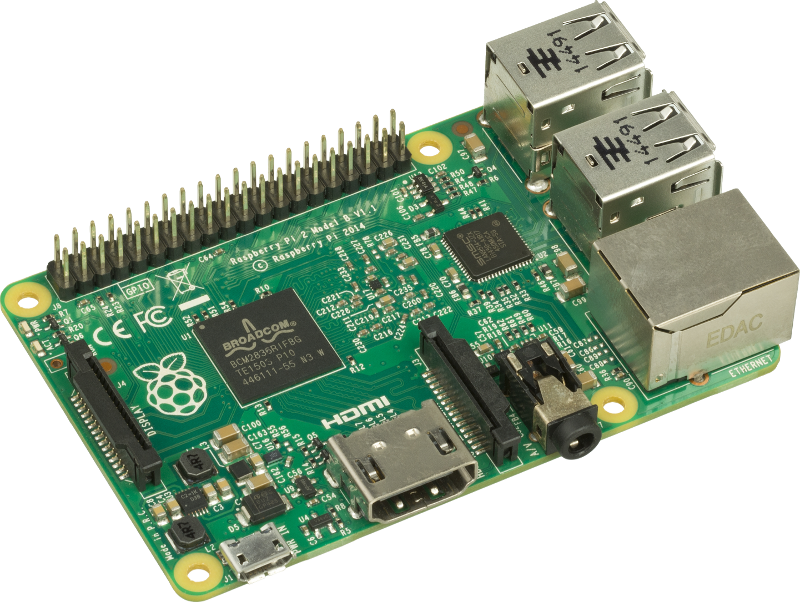
\includegraphics[width=0.56\textwidth]{res/raspberry}}
\caption{Raspberry Pi \cite{raspberry} with Broadcom System on Chip \label{fig:raspberry}}
\end{figure}
Actually almost all of the embedded systems use a SoC with similar boards, each one with its own size and configuration.

In order to accommodate different potential implementations, each pin (or group of pins) of a SoC may have multiple configuration and operating modes,
depending on the board they are attached to. The configuration of the pins is managed by the pin controller, a particular subsystem of any SoC.
Through the pin controller, the system can configure the operating mode of the pins, such as their input or output mode.
The features of a pin controller can be grouped into two main categories:
\begin{itemize}
	\item Pin configuration: allows the system to change some electrical properties of the pins (see \sec \ref{sec:iopins});
	\item Pin multiplexing: each pin of the SoC may have many usage usages, also known as \emph{alternate functions}, depending on what is needed by the external board.
		The pin multiplexing feature enables the system to specify which type of function is needed on each pin.
\end{itemize}
As the I/O attack is a very low-level attack, it is necessary to dig further into the electrical world to know how these I/O interfaces work.


\subsection{I/O pins}
\label{sec:iopins}

I/O interfaces of a System on Chip provides a connection between internal modules and external electronic devices.
As shown in \myfig{\ref{fig:chips}}, they are physically visible from the outside of the chip package,
usually in the form of pins \subref{fig:pins} or soldering balls \subref{fig:balls}.

\begin{figure}[h]
\centering

\begin{subfigure}{.45\textwidth}
\centering
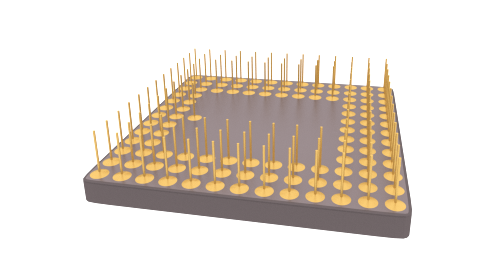
\includegraphics[width=\linewidth]{res/pins}
\caption{\label{fig:pins}}
\end{subfigure}
\begin{subfigure}{.45\textwidth}
\centering
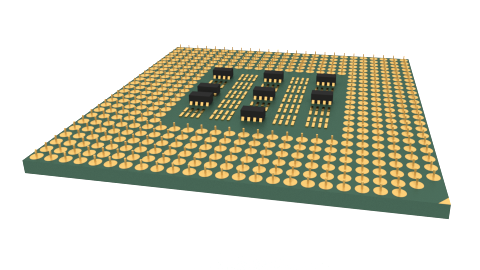
\includegraphics[width=\linewidth]{res/balls}
\caption{\label{fig:balls}}
\end{subfigure}

\caption{I/O connections packaged as \subref{fig:pins} Pin Grid Array and \subref{fig:balls} Ball Grid Array\label{fig:chips}}
\end{figure}

Internally they are connected to the silicon die through bonding wires, and are managed by a specific I/O circuit which may vary according to the specific chip.
Although there are many different implementations, almost all of the available SoCs have I/O ports with very similar functionalities.
For our purpose, we can describe them in an implementation-independent manner by using simplified generic schematics.


\subsubsection{Pin configuration}
\label{sec:pinconf}

The schematic depicted in \myfig{\ref{fig:pinconf}} helps us to discuss about the first set of features: pin configuration.
The operation mode described in this section is also known as General Purpose I/O (GPIO).

\begin{figure}[h]
\centerline{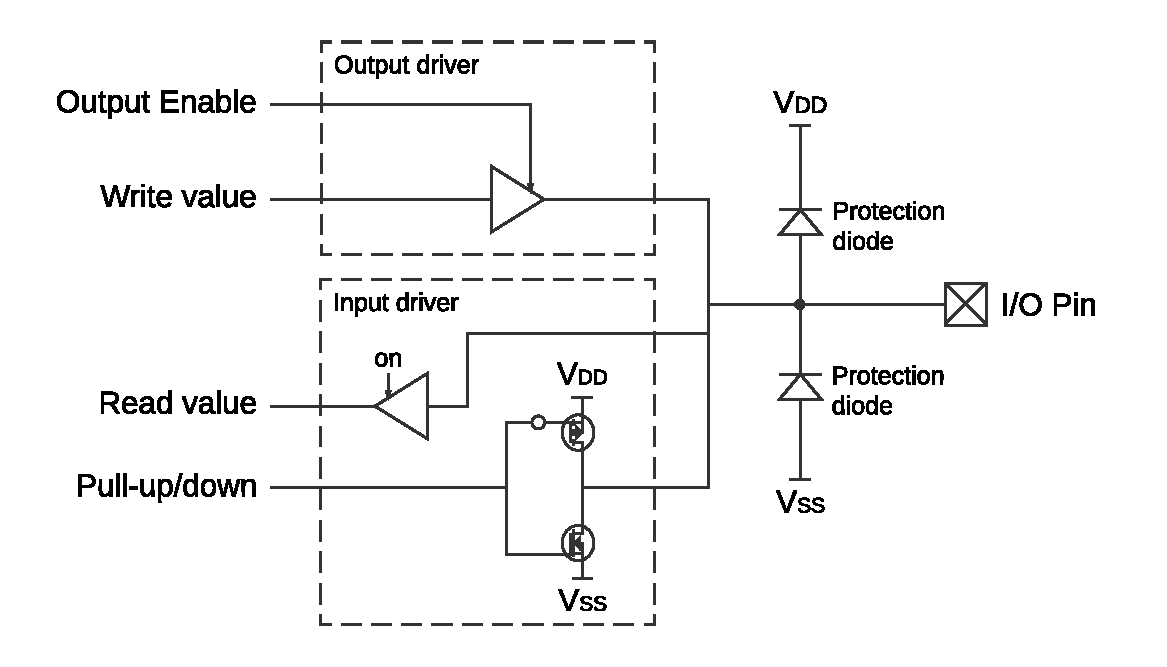
\includegraphics[width=0.8\textwidth]{res/pinconf}}
\caption{General Purpose I/O pin configuration circuit \label{fig:pinconf}}
\end{figure}

Apart from the protection diodes that serve as shield against input currents lower than $V_{SS}$ or higher than $V_{DD}$,
the circuit is divided into two different parts: one for output and one for input.
\begin{itemize}
	\item \itemname{Output driver}:
		The output module is basically a buffer controlled by an output enable signal.
		This signal controls the input or output mode of the pin. If it is high, then the pin is in output mode
		and the value coming from a write operation goes through the buffer to the actual pin.
		If it is low, the pin is in input mode and the write signal is blocked, so it is not possible to change the external value of the pin from inside anymore.
	\item \itemname{Input driver}:
		The input driver has a similar buffer to read the value, usually having hysteresis capability which is useful for filtering unstable external values.
		Since the read buffer is always active, the input value is always available, even if the pin is currently working in output mode.
		The reason for this is merely physical: even if the external value was blocked by the buffer,
		one would always get a value by reading the input signal, because a value is nothing but an interpretation of the voltage level on a wire.
		When the pin is set as input, the pull-up/pull-down network enables the user to have a ``default'' value on the pin,
		namely a defined state maintained while the pin is not actively driven from outside. This feature is useful to avoid so called ``floating'' inputs.
\end{itemize}

For Pin Control Attack, what is more interesting about the circuit in \myfig{\ref{fig:pinconf}} are the following two properties:
\begin{itemize}
	\item there is no checking about the input state, so it is possible to perform a read even when the pin is in output mode;
	\item vice versa, it is not possible to write to a pin which has been configured as output.
\end{itemize}

Furthermore, it is also possible to drive the pull-up/down network, factually disturbing the real value of the I/O pin in an unpredictable way.
In this case the effects strongly depends on the actual implementation of the circuit as well as on the capacitive load connected to the external I/O pin.


\subsubsection{Pin multiplexing}

Inside the chip an I/O pin may be connected to more than one device, which can be selected depending on the application,
that is the way of soldering or wiring the package into an electronic board.
This SoC feature is known as pin multiplexing (also ball multiplexing, pad multiplexing, alternate functions).
Even though pin multiplexing is designed for hardware configuration, in almost all modern chips it is possible to change the function at runtime.

\begin{figure}[h]
\centerline{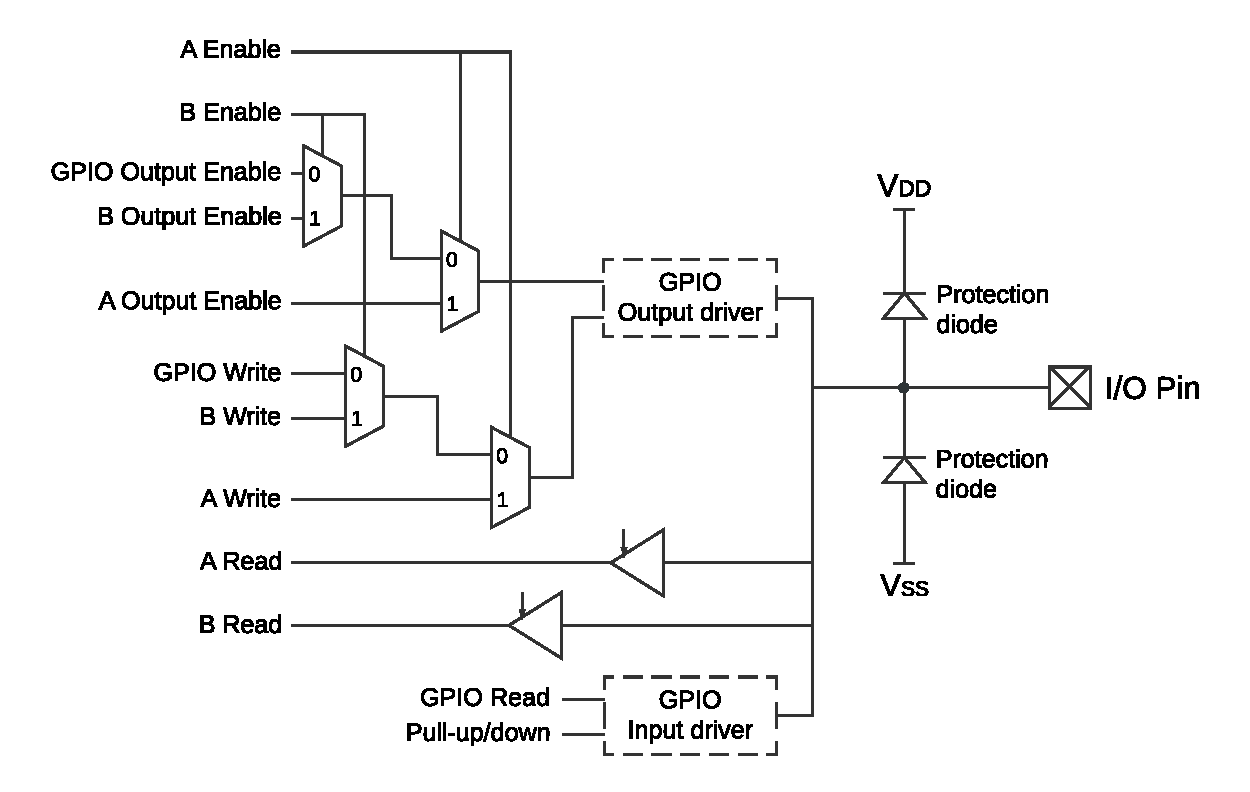
\includegraphics[width=0.8\textwidth]{res/pinmux}}
\caption{Generic I/O pin multiplexing circuit \label{fig:pinmux}}
\end{figure}

\myfig{\ref{fig:pinmux}}~ shows a possible hardware implementation of pin multiplexing.
The I/O pin in the figure is connected to two different peripherals inside the chip, namely A and B,
and it is also accessible through basic GPIO as described in \sec \ref{sec:pinconf} above.
The access to the GPIO output driver is regulated by two in cascade multiplexers for each signal of the module.
If the peripheral A is enabled, then the signals driven by A go through the multiplexers and can drive the actual value of the pin,
while GPIO and peripheral B output signals are blocked. Instead, if only peripheral B is enabled then only its signals are able to reach the I/O pin.
Note that in this last case the peripheral A should not be enabled, because A multiplexers have precedence against B ones.
Thus, the cascading of multiplexers actually implements a priority mechanism between peripherals A and B.
If neither A nor B are enabled, then no alternate function is active for the I/O pin and it could be driven by GPIO signals.
Each peripheral may also have its own dedicated input line, to get values from the I/O port in the same way as GPIO does.

For our purpose, at least two interesting properties can be inferred from pin multiplexing schematic of \myfig{\ref{fig:pinmux}}:
\begin{itemize}
	\item it is possible to block output signals from peripherals by simply changing the multiplexing configuration;
	\item the GPIO value can be read at any time, independently from the current multiplexing state of the output.
\end{itemize}


\section{Pin Control Attack}

TODO Continue with attack analysis and the rest of the chapter.


\chapter{Pin Control Protection}
\label{chap:design}

TODO Pin Control Protection design and implementation.



\chapter{Experimental Results}
\label{chap:results}

TODO Experimental Results.


\chapter{Conclusions}
\label{chap:conclusions}

This final chapter concludes the presented work, highlighting its main contribution and drawbacks, and suggesting possible future works.


\section{Contribution and drawbacks}
\label{sec:contrib}

The scientific contribution of this work is made of two main components:
\begin{enumerate}
	\item analyse I/O attack and prove that it is actually feasible on real PLCs;
	\item design and implement a possible countermeasure, achieving a good detection rate without causing an unacceptable performance overhead.
\end{enumerate}
Both parts can obviously be improved and continued, as discussed later in \mysec{sec:future}.

By analysing the attack, we demonstrated that it is possible to tamper with the I/O operations even in a real PLC architecture, where input/output is managed by external modules.
Furthermore, we were able to clearly define the requirements and the attack vectors available for the attacker, useful to abstract the problem and design a proper solution.
In the first part of \mychap{chap:defense}, we tried to define abstract strategies that could be applied to any embedded system to tackle any kind of I/O attack.
Furthermore, the implementation has been designed to minimise the effort required to adapt the solution to different systems and architectures.

Nevertheless, our detection system is still the first step against I/O attack, and, of course, it has some limitations.
First, it is not a complete solution, in the sense that I/O attacks could still be possible if the attacker is able to gain accurate timing precision and evade our time-based monitors.
Of course this raises the bar for the attacker, who has to conduct more elaborated attacks to achieve the same result.
Moreover, our detection monitors can be improved and optimized to increase their detection rate, factually discouraging any malicious attempt.
Second, an attacker who gains kernel level access may still be able to circumvent our defensive mechanism, and other techniques should be used in combination with it,
as previously discussed in \mysec{sec:def-sec}. In the next section we discuss some possible future works regarding both our contributions.


\section{Future works}
\label{sec:future}

During each phase of this work, many ideas about possible future works came out.
First, for the attack phase, further possibilities can be analysed to implement more elaborated attacks on the real PLC with external I/O modules.
For instance, in our Wago PLC, it may be possible to fake both input and output by leveraging SPI bitbanging technique.
A possible implementation of this attack can do the following:
\begin{itemize}
	\item synchronise itself with PLC I/O operation;
	\item disable next PLC I/O operation using one of the techniques presented in \mysec{sec:attack-plc};
	\item perform malicious I/O operation within the next scan cycle, \eg shifted by $\SI{5}{ms}$ after the real one (accurate synchronisation is required).
\end{itemize}
Note that all these operations can be done with the same assumptions made for the described I/O attack, without hooking any function nor modifying PLC logic/runtime.
Moreover, several vendors are currently producing different PLCs having a small subset of I/O interfaces directly available without the need of external modules.
If this feature, known as \emph{Integrated I/O}, is actively used on a control system, then the attacker can have direct access to sensors and actuators as well,
without needing to go through the additional level of indirection caused by external modules. In this case, the original version of Pin Control Attack would be applicable.

For the defense phase, many improvements and extension are doable.
First, detection rates of DR and I/O monitor can be improved by synchronising them with respect to the timing of the PLC scan cycle.
In fact, if they are triggered in proximity of each PLC I/O operation, detecting more sophisticated attacks becomes easier.
To get accurate results, this approach needs to be tested in a real-time system.
Of course, if the vendor decides to integrate the defense with the PLC runtime itself, this would be the optimal solution, because it can simply check I/O configuration
right before performing an I/O operation.

Another benefit deriving from an integration with the PLC runtime would be a significant simplification of our defense,
in particular when it has to check whether the I/O configuration is in line with the current PLC logic.
We largely discussed this aspect in \mysec{sec:io-design}. Briefly, if the PLC runtime is designed to be aware of the defense,
it can provide a simpler interface for Ghostbuster to check if a conflict between configuration and logic occurred.
In fact, in our prototype implementation, described in \mysec{sec:io-impl}, we leveraged reverse engineering techniques to collect the necessary information.

Additionally, our solution may be extended with a performance monitor, to cover a larger set of attacks and increase the overall detection rate.
We can argue that a performance-based mechanism would be effective on a PLC system, which executes the same operations at each scan cycle, thus, it is very stable.
As previously discussed in \mysec{sec:pre-analysis}, the operations performed by the PLC runtime when a new logic is uploaded should be excluded from the detection.
Again, an integration with the PLC runtime would be helpful to design this behaviour as well.
For instance, the performance monitor may be disabled and re-enabled by the PLC runtime process through authenticated commands sent to the defense module.
All these proposed approaches should be evaluated with respect to the overhead imposed to the system.

Finally, our entire solution can be deployed within a Trusted Execution Environment, such as ARM TrustZone \cite{trustzone}.
However, this approach may not be feasible due to the excessive CPU performance degradation to switch between secure and non-secure world.
Therefore, a carefully designed solution is required to minimise its overhead.



\begin{thebibliography}{99}

\bibitem{ghostplc}
A.Abbasi, M.Hashemi, E.Zambon, S.Etalle,
``Stealth Low-Level Manipulation of Programmable Logic Controllers I/O By Pin Control Exploitation'',
TODO Complete citation CRITIS Conference 2016.

\bibitem{pinctrl}
``Pin Control Subsystem'',
\url{https://www.kernel.org/doc/Documentation/pinctrl.txt}.

\bibitem{stuxnet}
N.Falliere, L.O Murchu, E.Chien,
``W32.Stuxnet  Dossier'',
Version 1.4, Febr. 2011.
Online: \url{http://www.symantec.com/content/en/us/enterprise/media/security_response/whitepapers/w32_stuxnet_dossier.pdf}.

\bibitem{io-command}
R.Grandgenett, W.Mahoney, R.Gandhi,
``Authentication Bypass and Remote Escalated I/O Command Attacks'',
CISR '15: Proceedings of the 10th Annual Cyber and Information Security Research Conference,
Oak Ridge, Tennesse (USA), April 7-9, 2015,
\doi{10.1145/2746266.2746268}.

\bibitem{taxonomy}
D.Papp, Z.Ma, L.Buttyan,
``Embedded systems security: Threats, vulnerabilities, and attack taxonomy''
Privacy, Security and Trust (PST) 13th Annual Conference,
Izmir (Turkey), July 21-23, 2015
pp.\ 145-152,
\doi{10.1109/PST.2015.7232966}.

\bibitem{firmware-mod}
Z.Basnight, J.Butts, J.Lopez Jr., T.Dube,
``Firmware modification attacks on programmable logic controllers'',
International Journal of Critical Infrastructure Protection,
Volume 6, Issue 2, June 2013,
pp.\ 76-84,
\doi{10.1016/j.ijcip.2013.04.004}.

\bibitem{ethernet-vuln}
D.Peck, D.Peterson,
``Leveraging ethernet card vulnerabilities in field devices'',
Proceedings of the SCADA Security Scientific Symposium,
Miami Beach, Florida (USA), Jan. 18-19, 2009,
pp.\ 1-19.

\bibitem{print-vuln}
A.Cui, M.Costello, S.J.Stolfo,
``When Firmware Modifications Attack: A Case Study of Embedded Exploitation'',
20th Annual Network \& Distributed System Security Symposium,
San Diego, California (USA), Febr. 24-27, 2013,
\doi{10.7916/D8P55NKB}.

\bibitem{dynamic-payload}
S.McLaughlin,
``On Dynamic Malware Payloads Aimed at Programmable Logic Controllers'',
In 6th USENIX Workshop on Hot Topics in Security,
2011.

\bibitem{sabot}
S.McLaughlin, P.McDaniel,
``SABOT: Specification-based Payload Generation for Programmable Logic Controllers'',
CCS '12: Proceedings of the 2012 ACM conference on Computer and Communications Security,
New York (USA), Oct. 16-18, 2012,
pp.\ 439-449,
\doi{10.1145/2382196.2382244}.

\bibitem{siemens-s7}
D.Beresford,
``Exploiting Siemens Simatic S7 PLCs'',
Black Hat USA 2011,
Las Vegas, Nevada (USA), Aug. 3-4, 2011.
Online: \url{https://media.blackhat.com/bh-us-11/Beresford/BH_US11_Beresford_S7_PLCs_WP.pdf}.

\bibitem{plc-network}
J.Klick, S.Lau, D.Marzin, J.Malchow, V.Roth,
``Internet-facing PLCs as a Network Backdoor'',
Proceedings of IEEE Conference on Communications and Network Security (CNS),
Florence (Italy), Sept. 28-30, 2015,
pp.\ 524-532,
\doi{10.1109/CNS.2015.7346865}.

\bibitem{abb-codesys}
ICS-CERT,
``ABB AC500 PLC Webserver CoDeSys Vulnerability'',
April 30, 2013.
Online: \url{https://ics-cert.us-cert.gov/advisories/ICSA-12-320-01}.

\bibitem{codesys-server}
ICS-CERT,
``3S CODESYS Gateway-Server Vulnerabilities (Update A)'',
March 13, 2014.
Online: \url{https://ics-cert.us-cert.gov/advisories/ICSA-13-050-01A}.

\bibitem{schneider-bof}
ICS-CERT,
``Schneider Electric Modicon M340 Buffer Overflow Vulnerability'',
Dec. 17, 2015.
Online: \url{https://ics-cert.us-cert.gov/advisories/ICSA-15-351-01}.

\bibitem{rockwell-vuln}
ICS-CERT,
``Rockwell Automation Micrologix 1100 and 1400 PLC Systems Vulnerabilities (Update A)'',
Oct. 27, 2015.
Online: \url{https://ics-cert.us-cert.gov/advisories/ICSA-15-300-03A}.

\bibitem{rockwell-vuln2}
ICS-CERT,
``Rockwell Automation MicroLogix 1100 PLC Overflow Vulnerability'',
Jan. 26, 2016.
Online: \url{https://ics-cert.us-cert.gov/advisories/ICSA-16-026-02}.

\bibitem{elcsoft-vuln}
ICS-CERT,
``Eaton ELCSoft Programming Software Memory Vulnerabilities'',
June 30, 2016.
Online: \url{https://ics-cert.us-cert.gov/advisories/ICSA-16-182-01}.

\bibitem{jop}
P.Chen, X.Xing, B.Mao, L.Xie,
``Return-oriented rootkit without returns (on the x86)''
ICICS 2010: 12th International Conference on Information and Communications Security,
Barcelona (Spain), Dec. 15-17, 2010,
pp.\ 340-354,
\doi{10.1007/978-3-642-17650-0_24}.

\bibitem{no-ret}
S.Checkoway, L.Davi, A.Dmitrienko, A.Sadeghi, H.Shacham, M.Winandy,
``Return-Oriented Programming without Returns'',
CCS '10: Proceedings of the 17th ACM conference on Computer and Communications Security,
Chicago, Illinois (USA), Oct. 4-8, 2010,
\doi{10.1145/1866307.1866370}.

\bibitem{scada-attacks}
R.E.Johnson,
``Survey of SCADA Security Challenges and Potential Attack Vectors'',
ICITST 2010: International Conference for Internet Technology and Secured Transactions,
London (UK), Nov. 8-11, 2010,
pp.\ 80-85.

\bibitem{scada-attacks2}
B.Miller, D.Rowe,
``A survey of SCADA and critical infrastructure incidents'',
RIIT '12: Proceedings of the 1st Annual conference on Research In Information Technology,
Calgary, Alberta (Canada), Oct. 10-13, 2012,
pp.\ 51-56,
\doi{10.1145/2380790.2380805}.

\bibitem{plc-security}
G.P.H.Sandaruwan, P.S.Ranaweera, V.A.Oleshchuk,
``PLC Security and Critical Infrastructure Protection'',
ICIIS 2013: IEEE 8th International Conference on Industrial and Information Systems,
Peradeniya (Sri Lanka), Dec. 17-20, 2013,
pp.\ 81-85,
\doi{10.1109/ICIInfS.2013.6731959}.

\bibitem{stuxnet-defense}
A.Clark, Q.Zhu, R.Poovendran, T.Başar,
``An Impact-Aware Defense against Stuxnet'',
ACC 2013: 1st American Control Conference,
Washington, DC (USA), June 17-19, 2013,
pp.\ 4140-4147,
\doi{10.1109/ACC.2013.6580475}.

\bibitem{semantic-defense}
D.Hadžiosmanović, R.Sommer, E.Zambon, P.H.Hartel,
``Through the Eye of the PLC: Semantic Security Monitoring for Industrial Processes'',
ACSAC '14: 30th Annual Computer Security Applications Conference,
New Orleans, LA (USA), Dec. 08-12, 2014,
pp.\ 126-135,
\doi{10.1145/2664243.2664277}.

\bibitem{confirm}
X.Wang, C.Konstantinou, M.Maniatakos, R.Karri, S.Lee, P.Robison, P.Stergiou, S.Kim,
``Malicious Firmware Detection with Hardware Performance Counters'',
IEEE Transactions on Multi-Scale Computing Systems,
Vol.\ 2, Issue 3,
July-Sept. 2016,
pp.\ 160-173,
\doi{10.1109/TMSCS.2016.2569467}.

\bibitem{trustzone}
ARM Limited,
``ARM Security Technology - Building a Secure System using TrustZone® Technology'',
2009.
Online: \url{http://infocenter.arm.com/help/topic/com.arm.doc.prd29-genc-009492c/PRD29-GENC-009492C_trustzone_security_whitepaper.pdf}.

\bibitem{trustlite}
P.Koeberl, S.Schulz, A.Sadeghi, V.Varadharajan,
``TrustLite: A Security Architecture for Tiny Embedded Devices'',
EuroSys '14: Proceedings of the Ninth European Conference on Computer Systems,
Amsterdam (Netherlands), April 13-16, 2014,
\doi{10.1145/2592798.2592824}.

\bibitem{tpm2}
A.Fuchs, C.Krau{\ss}, J.Repp,
``Advanced Remote Firmware Upgrades Using TPM 2.0'',
in the book ``ICT Systems Security and Privacy Protection: 31st IFIP TC 11 International Conference, SEC 2016, Ghent, Belgium, May 30 - June 1, 2016, Proceedings''
edited by J.Hoepman, S.Katzenbeisser,
Springer International Publishing, 2016,
pp.\ 276-289,
\doi{10.1007/978-3-319-33630-5_19}.

\bibitem{blockchain}
B.Lee, J.Lee,
``Blockchain-based secure firmware update for embedded devices in an Internet of Things environment'',
The Journal of Supercomputing, 2016,
pp.\ 1-16,
\doi{10.1007/s11227-016-1870-0}.

\bibitem{logic-analytics}
S.Zonouz, J.Rrushi, S.McLaughlin,
``Detecting Industrial Control Malware Using Automated PLC Code Analytics'',
IEEE Security \& Privacy,
Vol.\ 12, Issue 6,
Nov.-Dec. 2014,
pp.\ 40-47,
\doi{10.1109/MSP.2014.113}.

\bibitem{hypervisor-control}
L.Garcia, S.Zonouz, D.Wei, L.P.de Aguiar,
``Detecting PLC Control Corruption via On-Device Runtime Verification'',
Resilience Week (RWS),
Chicago, Illinois (USA), Aug. 16-18, 2016,
pp.\ 67-72,
\doi{10.1109/RWEEK.2016.7573309}.

\bibitem{symbiotes}
A.Cui, S.J.Stolfo,
``Defending Embedded Systems with Software Symbiotes'',
in the book ``Recent Advances in Intrusion Detection: 14th International Symposium, RAID 2011, Menlo Park, CA, USA, September 20-21, 2011. Proceedings'',
edited by R.Sommer, D.Balzarotti, G.Maier,
Springer Berlin Heidelberg, 2011,
pp.\ 358-377,
\doi{10.1007/978-3-642-23644-0_19}.

\bibitem{swatt}
A.Seshadri, A.Perrig, L.Doom, P.Khosla,
``SWATT: SoftWare-based ATTestation for embedded devices'',
Proceedings of IEEE Symposium on Security and Privacy,
Oakland, California (USA), May 9-12, 2004,
pp.\ 272-282,
\doi{10.1109/SECPRI.2004.1301329}.

\bibitem{swatt-difficulty}
C.Castelluccia, A.Francillon, D.Perito, C.Soriente,
``On the difficulty of software-based attestation of embedded devices'',
CCS'09: Proceedings of the 16th ACM Conference on Computer and Communications Security,
Chicago, Illinois (USA), Nov. 9-13, 2009,
pp.\ 400-409,
\doi{10.1145/1653662.1653711}.

\bibitem{power-fingerprinting}
C.A.Gonzalez, A.Hinton,
``Detecting Malicious Software Execution in Programmable Logic Controllers Using Power Fingerprinting'',
in the book ``Critical Infrastructure Protection VIII: 8th IFIP WG 11.10 International Conference, ICCIP 2014, Arlington, VA, USA, March 17-19, 2014, Revised Selected Papers'',
edited by J.Butts, S.Shenoi,
Springer Berlin Heidelberg, 2014,
pp.\ 15-27,
\doi{10.1007/978-3-662-45355-1_2}.

\bibitem{autoscopy}
J.Reeves, A.Ramaswamy, M.Locasto, S.Bratus, S.Smith,
``Intrusion detection for resource-constrained embedded control systems in the power grid'',
International Journal of Critical Infrastructure Protection, 2012,
Vol.\ 5, No.\ 2,
pp.\ 74-83,
\doi{10.1016/j.ijcip.2012.02.002}.

\bibitem{disarm}
J.Habibi, A.Panicker, A.Gupta, E.Bertino,
``DisARM: Mitigating Buffer Overflow Attacks on Embedded Devices'',
in the book ``Network and System Security: 9th International Conference, NSS 2015, New York, NY, USA, November 3-5, 2015, Proceedings'',
edited by M.Qiu, S.Xu, M.Yung, H.Zhang,
Springer International Publishing, 2015,
pp.\ 112-129,
\doi{10.1007/978-3-319-25645-0_8}.

\bibitem{hardware-ibmac}
A.Francillon, D.Perito, C.Castelluccia,
``Defending Embedded Systems Against Control Flow Attacks'',
SecuCode '09: Proceedings of the first ACM workshop on Secure execution of untrusted code,
Chicago, Illinois (USA), Nov. 9, 2009,
pp.\ 19-26,
\doi{10.1145/1655077.1655083}.

\bibitem{ocfmm}
F.Abad, J.Woude, Y.Lu, S.Bak, M.Caccamo, L.Sha, R.Mancuso, S.Mohan,
``On-Chip Control Flow Integrity Check for Real Time Embedded Systems'',
2013 IEEE 1st International Conference on Cyber-Physical Systems, Networks, and Applications (CPSNA),
Taipei, Taiwan, Aug. 19-20, 2013,
pp.\ 26-31,
\doi{10.1109/CPSNA.2013.6614242}.

\bibitem{fine-grained}
L.Davi, P.Koeberl, A.Sadeghi,
``Hardware-Assisted Fine-Grained Control-Flow Integrity: Towards Efficient Protection of Embedded Systems Against Software Exploitation'',
DAC '14: Proceedings of the 51st Annual Design Automation Conference,
San Francisco, California (USA), June 1-5, 2014,
pp.\ 133:1-133:6,
\doi{10.1109/DAC.2014.6881460}.

\bibitem{hafix}
L.Davi, M.Hanreich, D.Paul, A.Sadeghi, P.Koeberl, D.Sullivan, O.Arias, Y.Jin,
``HAFIX: Hardware-Assisted Flow Integrity Extension'',
DAC '15: Proceedings of the 52nd Annual Design Automation Conference,
San Francisco, California (USA), June 7-11, 2015,
pp.\ 74:1-74:6,
\doi{10.1145/2744769.2744847}.

\bibitem{bb-cfi}
S.Das, W.Zhang, Y.Liu,
``A Fine-Grained Control Flow Integrity Approach Against Runtime Memory Attacks for Embedded Systems'',
IEEE Transactions on Very Large Scale Integration (VLSI) Systems,
Vol.\ 24, No.\ 11,
Nov. 2016,
pp.\ 3193-3207,
\doi{10.1109/TVLSI.2016.2548561}.

\bibitem{cflat}
T.Abera, N.Asokan, L.Davi, J.Ekberg, T.Nyman, A.Paverd, A.Sadeghi, G.Tsudik,
``C-FLAT: Control-FLow ATtestation for Embedded Systems Software'',
CCS '16: Proceedings of the 23rd ACM Conference on Computer and Communications Security,
Vienna (Austria), Oct. 24-28, 2016,
pp.\ 743-754,
\doi{10.1145/2976749.2978358}.

\bibitem{smm-rootkit}
S.Embleton, S.Sparks, C.C.Zou,
``SMM rootkit: a new breed of OS independent malware'',
Security and Communication Networks,
Vol.\ 6, No.\ 12,
Dec. 2013,
pp.\ 1590-1605,
\doi{10.1002/sec.166}.

\bibitem{iocheck}
F.Zhang,
``IOCheck: A framework to enhance the security of I/O devices at runtime'',
43rd Annual IEEE/IFIP Conference on Dependable Systems and Networks Workshop (DSN-W),
Budapest (Hungary), June 24-27, 2013,
\doi{10.1109/DSNW.2013.6615523}.

\bibitem{raspberry}
Raspberry Pi Foundation,
``Raspberry Pi'',
\url{https://www.raspberrypi.org/}.

\bibitem{symbiote_web}
Red ballon security,
``Symbiote Defense'',
\url{http://www.redballoonsecurity.com}.

\bibitem{autoscopy_web}
Trustworthy Cyber Infrastructure for the Power Grid,
``Autoscopy Jr.'',
\url{https://tcipg.org/technology/autoscopy-jr}.

\bibitem{bcm2835}
Raspberry Pi Foundation,
``BCM2835'',
\url{https://www.raspberrypi.org/documentation/hardware/raspberrypi/bcm2835/README.md}.

\bibitem{codesys_runtime}
3S-Smart Software Solutions GmbH,
``CODESYS Control for Raspberry Pi SL'',
\url{http://store.codesys.com/codesys-control-for-raspberry-pi-sl.html}.

\bibitem{codesys_dev}
3S-Smart Software Solutions GmbH,
``CODESYS Development System V3'',
\url{http://store.codesys.com/codesys.html}.

\bibitem{wago_linux}
WAGO Kontakttechnik GmbH \& Co.,
``Linux - Automation for the Future'',
\url{http://global.wago.com/en/products/new-items/overview/basic-page-2600.jsp}.

\bibitem{am35x}
Texas Instruments,
``AM3517 Sitara Processor Technical documents'',
\url{http://www.ti.com/product/AM3517/technicaldocuments}.

\bibitem{strace}
``strace: Linux syscall tracer'',
\url{https://strace.io/}.

\bibitem{kprobes}
J.Keniston, P.S.Panchamukhi, M.Hiramatsu,
``Kernel probes'',
\url{https://www.kernel.org/doc/Documentation/kprobes.txt}.

\end{thebibliography}



%\begin{appendices}
%\setcounter{table}{0}
%\setcounter{figure}{0}
%\renewcommand\thetable{\thesection\arabic{table}}
%\renewcommand\thefigure{\thesection\arabic{figure}}

%\end{appendices}


\end{document}
